\documentclass[a4paper]{article}
\usepackage[utf8]{inputenc} % para poder usar tildes en archivos UTF-8
\usepackage[spanish]{babel} % para que comandos como \today den el resultado en castellano
\usepackage{a4wide} % márgenes un poco más anchos que lo usual
\usepackage[showRevisiones]{caratula}
\usepackage{xcolor}
\usepackage{listings}
\lstset{basicstyle=\ttfamily,
  showstringspaces=false,
  commentstyle=\color{red},
  keywordstyle=\color{blue}
}

\begin{document}

\materia{Organización de Computadoras 66.20}
\tipoapunte{Trabajo Práctico #0}

\fecha{\today}

\autor{Flórez Del Carpio, Christian}{91011}{chris.florez.d.c@gmail.com}
\autor{Montenegro, Josefina}{94289}{mariajosefina.mont@gmail.com}
\autor{Quino López, Julián}{94224}{julianquino2@gmail.com}

\revision{05/09/2017}{-}{Entrega primera versión del TP}
\revision{12/09/2017}{Luciano}{Correcciones varias}
\revision{26/09/2017}{Luciano}{Entrega del TP con correcciones}
\revision{09/09/2017}{Luciano}{2da entrega del TP con correcciones}
\maketitle

\begin{abstract}
El siguiente trabajo práctico tiene como objetivo familiarizarse con las herramientas mencionadas en el curso, para lograr tal propósito se debe determinar para un conjunto de palabras cuáles de ellas son palíndromos, entendiendo como palabras a aquellas compuestas por letras [A-Z], números [0-9], guiones bajos y medios, es decir, cualquier combinación posible de los anteriormente mencionados. Este programa debe correrse en la arquitectura MIPS32.
\end{abstract}


\section{Introducción}
Pueden haber tres escenarios posibles, el caso en el cual el usuario ingresa archivo de entrada y salida, el caso en el que se ingresa un archivo de entrada solamente y por último el caso donde se recibe el archivo de salida. En caso de no proporcionar un archivo de texto como entrada, se requerirá ingresar el stream por entrada standard. Si no se especifica un archivo de salida, se mostrarán los resultados por salida standard. 


\section{Desarrollo}

El algoritmo propuesto por el grupo consiste en parsear las palabras ingresadas para luego procesar una por una y decidir si son palíndromos o no, esto se realiza ya sea desde el archivo o utilizando el stream leído por entrada standard. Cabe destacar que tanto los archivos ingresados por el usuario como la entrada (stdin) y salida standard (stdout), respectivamente, son procesados de la misma forma.

\subsection{Comandos para compilar y ejecutar el programa}

Se puede compilar el programa con el siguiente comando:

\begin{lstlisting}[language=bash]
  $ gcc isPalindrome.c -o tp0
\end{lstlisting}


Y luego ejecutarlo con el comando:

\begin{lstlisting}[language=bash]
  $ ./tp0 -i input.txt -o output.txt
\end{lstlisting}

En caso de sólo querer especificar el archivo de entrada, debe ejecutarse, por ejemplo, de la siguiente manera:

\begin{lstlisting}[language=bash]
  $ ./tp0 -i input.txt -o -
\end{lstlisting}

Análogamente si se quiere ingresar un archivo de salida:

\begin{lstlisting}[language=bash]
  $ ./tp0 -i - -o output.txt
\end{lstlisting}

Es decir que con un guión medio indicamos que no se proporcionará un archivo para entrada/salida, acorde a lo que indica el enunciado.

Por otro lado, si no se desea ingresar ningún argumento y se desea trabajar con los streams de entrada y salida standard, debe ejecutarse de la siguiente forma:

\begin{lstlisting}[language=bash]
  $ ./tp0
\end{lstlisting}

\subsection{Otros comandos}

Pueden utilizarse comandos tales como help y version, de la siguiente forma:

\begin{lstlisting}[language=bash]
  $ ./tp0 -h
\end{lstlisting}

\begin{lstlisting}[language=bash]
  $ ./tp0 -V
\end{lstlisting}

\subsection{Código fuente}
\begin{lstlisting}[language=C]
#include <stdio.h>
#include <string.h>
#include <ctype.h>
#include <getopt.h>
#include <stdbool.h>
#include <stdlib.h>
#include <errno.h>
#include <unistd.h>

#define ERROR -1
#define SALIDA_EXITOSA 0

/**
 *
 * @param palabra a analizar
 * @return si la palabra es palíndroma o no
 */
bool isPalindrome(char *palabra) {
    int posInicial, posFinal;
    posFinal = strlen(palabra) - 1;
    for (posInicial = 0; posInicial < strlen(palabra) / 2; posInicial++, posFinal--) {
        if ((toupper(*(palabra + posInicial))) != (toupper(*(palabra + posFinal)))) {
            return false;
        }
    }
    return true;
}

/**
 *
 * @param palabras a analizar
 * @param archivo de salida
 * @param cantidadPalabras
 * @return un código
 */
int seekPalindromes(char **palabras, FILE *archivo, int cantidadPalabras) {
    int contadorPalabra = 0;
    while (contadorPalabra<cantidadPalabras) {
        if (isPalindrome(palabras[contadorPalabra])) {
            if (fputs(palabras[contadorPalabra], archivo) == EOF) {
                fprintf(stderr, "Error fputs: %s\n", strerror(errno));
                return ERROR;
            }
            if (fputs("\n", archivo)==EOF) {
                fprintf(stderr, "Error fputs: %s\n", strerror(errno));
                return ERROR;
            }
        }
        free(palabras[contadorPalabra]);
        contadorPalabra++;
    }
    return SALIDA_EXITOSA;
}

/**
 *
 * @param character
 * @return si el caracter es válido
 */
bool validCharacter(char character) {
    int asciiNumber = (int) character;
    if ((asciiNumber <= 57) && (asciiNumber >= 48)) {
        return true;
    }
    if ((asciiNumber <= 90) && (asciiNumber >= 65)) {
        return true;
    }
    if ((asciiNumber <= 122) && (asciiNumber >= 97)) {
        return true;
    }
    if (asciiNumber == 45) {
        return true;
    }
    if (asciiNumber == 95) {
        return true;
    }
    return false;
}

/**
 *
 * @param caracter
 * @param vector
 * @param contador
 * @return una palabra parcial
 */
char *agregarCaracterAVector(char caracter, char *vector, int contador){
    char *cadena = NULL;
    if(contador == 1){
        cadena = malloc(contador*sizeof(char));
        cadena[0] = caracter;

    }else{
        cadena = realloc(vector, contador * sizeof(char));
        cadena[contador-1]=caracter;
    }
    return cadena;
}

/**
 *
 * @param palabra
 * @param palabras
 * @param contDePalabrasGuardadas
 * @return un vector de palabras
 */
char **agregarPalabraAVector(char *palabra,char **palabras,int contDePalabrasGuardadas){
    char **auxiPalabras=NULL;
    if (contDePalabrasGuardadas == 1) {
        auxiPalabras = malloc(contDePalabrasGuardadas*sizeof(char*));
        auxiPalabras[0] = palabra;
    } else {
        auxiPalabras = realloc(palabras, contDePalabrasGuardadas * sizeof(char*));
        auxiPalabras[contDePalabrasGuardadas-1] = palabra;
    }
    return auxiPalabras;
}

/**
 *
 * @param contador
 * @param archivo
 * @return una línea leída del archivo
 */
char* getLinea(int* contador, FILE* archivo) {
    int letra;
    int finDeLinea ='\n';
    char* vector = NULL;
    letra = fgetc(archivo);
    while (!feof(archivo) && letra != finDeLinea) {
        (*contador)++;
        vector = (char*)realloc(vector,(*contador) *sizeof(char));
        vector[*contador-1]  = (char)letra;
        letra = fgetc(archivo);
    }

    (*contador)++;
    vector = (char*)realloc(vector,(*contador) *sizeof(char));
    vector[*contador-1]  = '\0';

    return vector;
}

/**
 *
 * @param linea
 * @param tamanioLinea
 * @param cantidadPalabras
 * @return todas las palabras de la línea
 */
char** parseLine(char *linea, int tamanioLinea, int *cantidadPalabras){
    char **palabras= NULL;
    char *palabra = NULL;
    int contador = 0;
    int contDePalabrasGuardadas = 0;
    int contDeCaracteresGuardados = 0;
    while (contador < tamanioLinea) {
        if (validCharacter(linea[contador])) {
            contDeCaracteresGuardados++;
            palabra = agregarCaracterAVector(linea[contador], palabra,contDeCaracteresGuardados);
        }else if (contDeCaracteresGuardados != 0) {
            contDeCaracteresGuardados++;
            contDePalabrasGuardadas++;
            palabra = agregarCaracterAVector('\0', palabra,contDeCaracteresGuardados);
            palabras = agregarPalabraAVector(palabra,palabras,contDePalabrasGuardadas);
            contDeCaracteresGuardados=0;
        }
        contador++;
    }
    *cantidadPalabras = contDePalabrasGuardadas;
    return palabras;
}

/**
 * Procesa el archivo de entrada o el stream ingresado por stdin
 *
 * @param inputFile
 * @param outputFile
 * @return un código
 */
int processInput(FILE *inputFile, FILE *outputFile) {
    char* bufferLinea = NULL;
    int tamanioLinea = 0;
    char **palabras = NULL;
    int cantidadPalabras = 0;
    // para reposicionar el puntero del archivo a la primera linea
    // lectura anticipada del archivo para q no de mas lecturas
    bufferLinea = getLinea(&tamanioLinea, inputFile);

    while (!feof(inputFile)) {
        palabras = parseLine(bufferLinea,tamanioLinea,&cantidadPalabras);  // carga en la matriz las palabras
        free (bufferLinea);
        bufferLinea = NULL;
        tamanioLinea = 0;
        if (seekPalindromes(palabras, outputFile,cantidadPalabras) == ERROR) {
            return ERROR;
        }
        bufferLinea = getLinea(&tamanioLinea, inputFile);
    } 
    if(fclose(inputFile)==EOF){
        fprintf(stderr, "Error fclose: %s\n", strerror( errno ));
        return ERROR;
    }

    if(outputFile != stdout){
        if(fclose(outputFile)==EOF){
            fprintf(stderr, "Error fclose: %s\n", strerror( errno));
            return ERROR;
        }
    }

    return SALIDA_EXITOSA;
}

int main(int argc, char *argv[]) {
    int option = 0;
    const char *short_opt = "i:o:hV";
    struct option long_opt[] = {
            {"version", no_argument,       NULL, 'V'},
            {"help",    no_argument,       NULL, 'h'},
            {"input",   required_argument, NULL, 'i'},
            {"output",  required_argument, NULL, 'o'},
            {NULL, 0,                      NULL, 0}
    };
    FILE *inputFile = NULL;
    FILE *outputFile = NULL;

    while ((option = getopt_long(argc, argv, short_opt, long_opt, NULL)) != -1) {
        switch (option) {
            case 'V':
                printf("TP #0 de la materia Organización de Computadoras \n");
                printf("Alumnos: \n");
                printf("    Flórez Del Carpio Christian\n   Montenegro Josefina \n  Quino Lopez Julian \n");
                return 0;
            case 'h':
                printf("Usage: \n");
                printf("    %s -h \n", argv[0]);
                printf("    %s -V \n", argv[0]);
                printf("    %s [options] \n", argv[0]);
                printf("Options: \n");
                printf("    -V, --version  Print version and quit. \n");
                printf("    -h, --help     Print this information. \n");
                printf("    -o, --output   Location of the output file. \n");
                printf("    -i, --input    Location of the input file. \n");
                return 0;
            case 'i':
                inputFile = fopen(optarg, "r");
                if (inputFile == NULL) {
                    fprintf(stderr, "Error archivo entrada: %s\n", strerror(errno));
                }
                break;
            case 'o':
                // verifico si existe el archivo
                if (access(optarg, W_OK) != -1) {
                    outputFile = fopen(optarg, "w+");
                    if (outputFile == NULL) {
                        fprintf(stderr, "Error archivo salida: %s\n", strerror(errno));
                        return ERROR;
                    }
                }
                break;
            default:
                // así está en el manual de getopt
                abort();
        }
    }

    if (inputFile == NULL) {
        inputFile = stdin;
    }

    if (outputFile == NULL) {
        outputFile = stdout;
    }

    if (processInput(inputFile, outputFile) == ERROR) {
        return ERROR;
    }

    return SALIDA_EXITOSA;
}

\end{lstlisting}

\subsection{Documentación detallada de las funciones presentadas en el código}

\paragraph{Función isPalindrome:}
Recibe por parámetro una palabra previamente filtrada, y analiza si la misma es palíndroma o no.

\paragraph{Función seekPalindromes:}
Recibe las palabras filtradas, el archivo donde escribir, evalúa si las palabras recibidas son palíndromos y en tal caso, las escribe en el archivo de salida.

\paragraph{Función validCharacter:}
Recibe un caracter y retorna si el mismo es válido.

\paragraph{Función agregarCaracterAVector:}
Se agregan caracteres que forman una palabra.

\paragraph{Función agregarPalabraAVector:}
Se agregan las palabras filtradas al vector de palabras.

\paragraph{Función getLinea:}
Devuelve una línea del archivo de entrada.

\paragraph{Función parseLine:}
Devuelve las palabras filtradas de una línea.

\paragraph{Función processInput:}
Procesa todas las líneas del archivo de entrada.

\section{Casos de prueba}

A continuación se muestran unos casos de prueba desde la consola del GXEmul, los textos utilizados se detallarán al final.


\begin{figure}[!htp]
\begin{center}
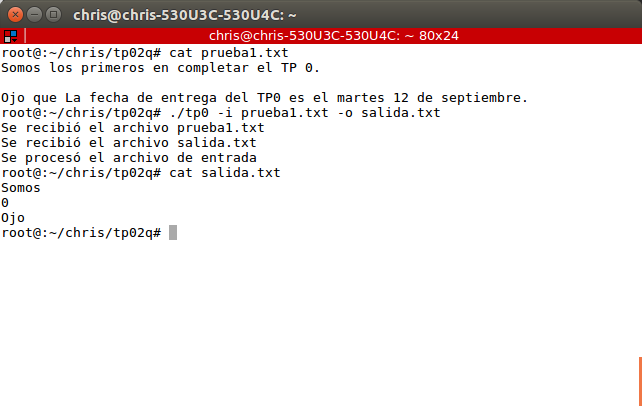
\includegraphics[width=0.5\textwidth]{prueba1.png}
\caption{Prueba utilizando archivo de entrada y salida.} \label{fig001}
\end{center}
\end{figure}

\begin{figure}[!htp]
\begin{center}
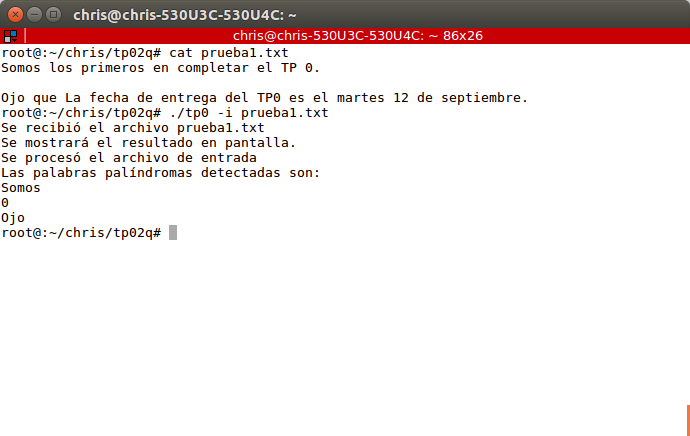
\includegraphics[width=0.5\textwidth]{prueba1SalidaPorPantalla.png}
\caption{Prueba utilizando solamente archivo de entrada.} \label{fig001}
\end{center}
\end{figure}

\begin{figure}[!htp]
\begin{center}
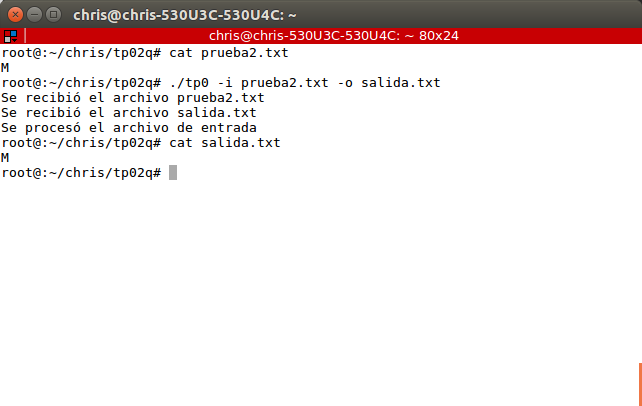
\includegraphics[width=0.5\textwidth]{prueba2.png}
\caption{Otra prueba utilizando otro archivo de entrada y salida.} \label{fig001}
\end{center}
\end{figure}

\begin{figure}[!htp]
\begin{center}
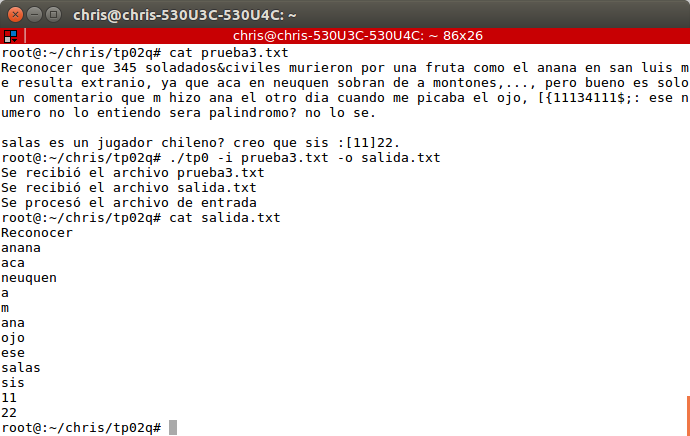
\includegraphics[width=0.5\textwidth]{prueba3.png}
\caption{Prueba utilizando otro archivo de entrada y salida.} \label{fig001}
\end{center}
\end{figure}

\begin{figure}[!htp]
\begin{center}
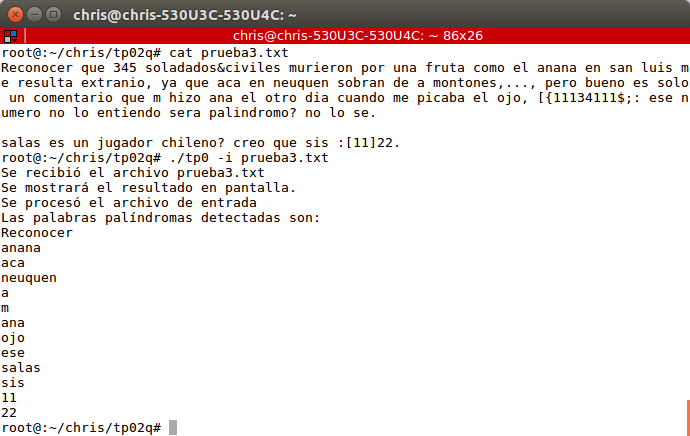
\includegraphics[width=0.5\textwidth]{prueba3salidaPorPantalla.png}
\caption{Prueba utilizando otro archivo de entrada.} \label{fig001}
\end{center}
\end{figure}

\begin{figure}[!htp]
\begin{center}
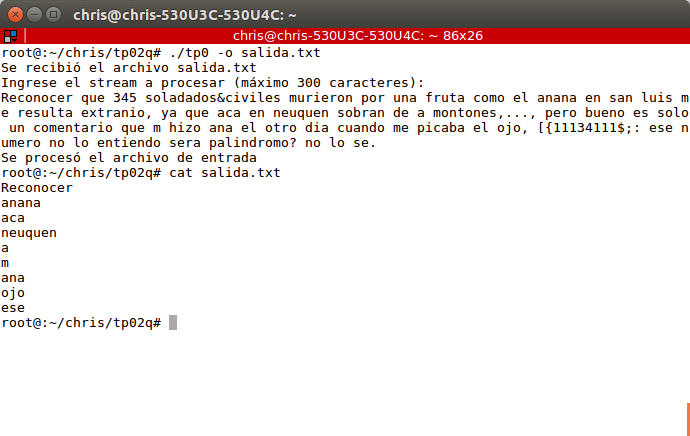
\includegraphics[width=0.5\textwidth]{pruebaPorTeclado.png}
\caption{Prueba utilizando solamente archivo de salida.} \label{fig001}
\end{center}
\end{figure}

\pagebreak

\subsection{Cobertura de los casos de prueba mencionados anteriormente}
\begin{enumerate}
\item En este caso se quiso probar que el programa no es case sensitive, lo cual lo hace bien ya que la palabra "Ojo" es dectectada como un palíndromo, y también se prueba que se guarda correctamente en el archivo de salida.
\item En este caso se proporciona sólo un archivo de entrada, el cual el programa procesa correctamente y al no especificar un archivo de salida se usa la salida standard de forma correcta para mostrar los resultados. 
\item En este caso se prueba que el programa detecta como palíndromo a una palabra compuesta por un solo caracter.
\item En este caso se prueba ingresando un archivo de entrada y salida que el programa detecta como caracteres separadores a todos aquellos que no fueran todas las letras del alfabeto (mayúsculas y minúsculas), números del 0 al 9, guión medio y guión bajo y que tambien detecta a los números 11 y 22 como palíndromos.
\item En este caso se prueba con un archivo de entrada más largo y sin especificar un archivo de salida, por lo que el programa imprime satisfactoriamente por pantalla el resultado.
\item En este caso se prueba que al ingresar un texto por entrada standard y especificando un archivo de salida, el programa procesa correctamente los datos y los escribe en el archivo de salida.
\end{enumerate}

\subsection{Textos utilizados}

\paragraph{Prueba 1:}

Somos los primeros en completar el TP 0.

Ojo que La fecha de entrega del TP0 es el martes 12 de septiembre.

\paragraph{Prueba 2:}

M

\paragraph{Prueba 3:} 

Reconocer que 345 soladados&civiles murieron por una fruta como el anana en san luis me resulta extranio, ya que aca en neuquen sobran de a montones,..., pero bueno es solo un comentario que m hizo ana el otro dia cuando me picaba el ojo, [{11134111\$;: ese numero no lo entiendo sera palindromo? no lo se.

salas es un jugador chileno? creo que sis :[11]22.

\pagebreak
    
\section{Código MIPS generado} 

\subsection{Código fuente Assembly}
\begin{lstlisting}[language=Assembler]
        .file   1 "isPalindrome.c"
    .section .mdebug.abi32
    .previous
    .abicalls
    .text
    .align  2
    .globl  isPalindrome
    .ent    isPalindrome
isPalindrome:
    .frame  $fp,56,$ra      # vars= 16, regs= 3/0, args= 16, extra= 8
    .mask   0xd0000000,-8
    .fmask  0x00000000,0
    .set    noreorder
    .cpload $t9
    .set    reorder
    subu    $sp,$sp,56
    .cprestore 16
    sw  $ra,48($sp)
    sw  $fp,44($sp)
    sw  $gp,40($sp)
    move    $fp,$sp
    sw  $a0,56($fp)
    lw  $a0,56($fp)
    la  $t9,strlen
    jal $ra,$t9
    addu    $v0,$v0,-1
    sw  $v0,28($fp)
    sw  $zero,24($fp)
$L18:
    lw  $a0,56($fp)
    la  $t9,strlen
    jal $ra,$t9
    srl $v1,$v0,1
    lw  $v0,24($fp)
    sltu    $v0,$v0,$v1
    bne $v0,$zero,$L21
    b   $L19
$L21:
    lw  $v1,56($fp)
    lw  $v0,24($fp)
    addu    $v0,$v1,$v0
    lb  $v0,0($v0)
    sll $v1,$v0,1
    lw  $v0,_toupper_tab_
    addu    $v0,$v1,$v0
    addu    $a0,$v0,2
    lw  $v1,56($fp)
    lw  $v0,28($fp)
    addu    $v0,$v1,$v0
    lb  $v0,0($v0)
    sll $v1,$v0,1
    lw  $v0,_toupper_tab_
    addu    $v0,$v1,$v0
    addu    $v0,$v0,2
    lh  $v1,0($a0)
    lh  $v0,0($v0)
    beq $v1,$v0,$L20
    sw  $zero,32($fp)
    b   $L17
$L20:
    lw  $v0,24($fp)
    addu    $v0,$v0,1
    sw  $v0,24($fp)
    lw  $v0,28($fp)
    addu    $v0,$v0,-1
    sw  $v0,28($fp)
    b   $L18
$L19:
    li  $v0,1           # 0x1
    sw  $v0,32($fp)
$L17:
    lw  $v0,32($fp)
    move    $sp,$fp
    lw  $ra,48($sp)
    lw  $fp,44($sp)
    addu    $sp,$sp,56
    j   $ra
    .end    isPalindrome
    .size   isPalindrome, .-isPalindrome
    .rdata
    .align  2
$LC0:
    .ascii  "Error fputs: %s\n\000"
    .align  2
$LC1:
    .ascii  "\n\000"
    .text
    .align  2
    .globl  seekPalindromes
    .ent    seekPalindromes
seekPalindromes:
    .frame  $fp,48,$ra      # vars= 8, regs= 3/0, args= 16, extra= 8
    .mask   0xd0000000,-8
    .fmask  0x00000000,0
    .set    noreorder
    .cpload $t9
    .set    reorder
    subu    $sp,$sp,48
    .cprestore 16
    sw  $ra,40($sp)
    sw  $fp,36($sp)
    sw  $gp,32($sp)
    move    $fp,$sp
    sw  $a0,48($fp)
    sw  $a1,52($fp)
    sw  $a2,56($fp)
    sw  $zero,24($fp)
$L24:
    lw  $v0,24($fp)
    lw  $v1,56($fp)
    slt $v0,$v0,$v1
    bne $v0,$zero,$L26
    b   $L25
$L26:
    lw  $v0,24($fp)
    sll $v1,$v0,2
    lw  $v0,48($fp)
    addu    $v0,$v1,$v0
    lw  $a0,0($v0)
    la  $t9,isPalindrome
    jal $ra,$t9
    beq $v0,$zero,$L27
    lw  $v0,24($fp)
    sll $v1,$v0,2
    lw  $v0,48($fp)
    addu    $v0,$v1,$v0
    lw  $a0,0($v0)
    lw  $a1,52($fp)
    la  $t9,fputs
    jal $ra,$t9
    move    $v1,$v0
    li  $v0,-1          # 0xffffffffffffffff
    bne $v1,$v0,$L28
    la  $t9,__errno
    jal $ra,$t9
    lw  $a0,0($v0)
    la  $t9,strerror
    jal $ra,$t9
    la  $a0,__sF+176
    la  $a1,$LC0
    move    $a2,$v0
    la  $t9,fprintf
    jal $ra,$t9
    li  $v0,-1          # 0xffffffffffffffff
    sw  $v0,28($fp)
    b   $L23
$L28:
    la  $a0,$LC1
    lw  $a1,52($fp)
    la  $t9,fputs
    jal $ra,$t9
    move    $v1,$v0
    li  $v0,-1          # 0xffffffffffffffff
    bne $v1,$v0,$L27
    la  $t9,__errno
    jal $ra,$t9
    lw  $a0,0($v0)
    la  $t9,strerror
    jal $ra,$t9
    la  $a0,__sF+176
    la  $a1,$LC0
    move    $a2,$v0
    la  $t9,fprintf
    jal $ra,$t9
    li  $v0,-1          # 0xffffffffffffffff
    sw  $v0,28($fp)
    b   $L23
$L27:
    lw  $v0,24($fp)
    sll $v1,$v0,2
    lw  $v0,48($fp)
    addu    $v0,$v1,$v0
    lw  $a0,0($v0)
    la  $t9,free
    jal $ra,$t9
    lw  $v0,24($fp)
    addu    $v0,$v0,1
    sw  $v0,24($fp)
    b   $L24
$L25:
    sw  $zero,28($fp)
$L23:
    lw  $v0,28($fp)
    move    $sp,$fp
    lw  $ra,40($sp)
    lw  $fp,36($sp)
    addu    $sp,$sp,48
    j   $ra
    .end    seekPalindromes
    .size   seekPalindromes, .-seekPalindromes
    .align  2
    .globl  validCharacter
    .ent    validCharacter
validCharacter:
    .frame  $fp,32,$ra      # vars= 16, regs= 2/0, args= 0, extra= 8
    .mask   0x50000000,-4
    .fmask  0x00000000,0
    .set    noreorder
    .cpload $t9
    .set    reorder
    subu    $sp,$sp,32
    .cprestore 0
    sw  $fp,28($sp)
    sw  $gp,24($sp)
    move    $fp,$sp
    move    $v0,$a0
    sb  $v0,8($fp)
    lb  $v0,8($fp)
    sw  $v0,12($fp)
    lw  $v0,12($fp)
    slt $v0,$v0,58
    beq $v0,$zero,$L31
    lw  $v0,12($fp)
    slt $v0,$v0,48
    bne $v0,$zero,$L31
    li  $v0,1           # 0x1
    sw  $v0,16($fp)
    b   $L30
$L31:
    lw  $v0,12($fp)
    slt $v0,$v0,91
    beq $v0,$zero,$L32
    lw  $v0,12($fp)
    slt $v0,$v0,65
    bne $v0,$zero,$L32
    li  $v0,1           # 0x1
    sw  $v0,16($fp)
    b   $L30
$L32:
    lw  $v0,12($fp)
    slt $v0,$v0,123
    beq $v0,$zero,$L33
    lw  $v0,12($fp)
    slt $v0,$v0,97
    bne $v0,$zero,$L33
    li  $v0,1           # 0x1
    sw  $v0,16($fp)
    b   $L30
$L33:
    lw  $v1,12($fp)
    li  $v0,45          # 0x2d
    bne $v1,$v0,$L34
    li  $v0,1           # 0x1
    sw  $v0,16($fp)
    b   $L30
$L34:
    lw  $v1,12($fp)
    li  $v0,95          # 0x5f
    bne $v1,$v0,$L35
    li  $v0,1           # 0x1
    sw  $v0,16($fp)
    b   $L30
$L35:
    sw  $zero,16($fp)
$L30:
    lw  $v0,16($fp)
    move    $sp,$fp
    lw  $fp,28($sp)
    addu    $sp,$sp,32
    j   $ra
    .end    validCharacter
    .size   validCharacter, .-validCharacter
    .align  2
    .globl  agregarCaracterAVector
    .ent    agregarCaracterAVector
agregarCaracterAVector:
    .frame  $fp,48,$ra      # vars= 8, regs= 3/0, args= 16, extra= 8
    .mask   0xd0000000,-8
    .fmask  0x00000000,0
    .set    noreorder
    .cpload $t9
    .set    reorder
    subu    $sp,$sp,48
    .cprestore 16
    sw  $ra,40($sp)
    sw  $fp,36($sp)
    sw  $gp,32($sp)
    move    $fp,$sp
    move    $v0,$a0
    sw  $a1,52($fp)
    sw  $a2,56($fp)
    sb  $v0,24($fp)
    sw  $zero,28($fp)
    lw  $v1,56($fp)
    li  $v0,1           # 0x1
    bne $v1,$v0,$L37
    lw  $a0,56($fp)
    la  $t9,malloc
    jal $ra,$t9
    sw  $v0,28($fp)
    lw  $v1,28($fp)
    lbu $v0,24($fp)
    sb  $v0,0($v1)
    b   $L38
$L37:
    lw  $a0,52($fp)
    lw  $a1,56($fp)
    la  $t9,realloc
    jal $ra,$t9
    sw  $v0,28($fp)
    lw  $v1,28($fp)
    lw  $v0,56($fp)
    addu    $v0,$v1,$v0
    addu    $v1,$v0,-1
    lbu $v0,24($fp)
    sb  $v0,0($v1)
$L38:
    lw  $v0,28($fp)
    move    $sp,$fp
    lw  $ra,40($sp)
    lw  $fp,36($sp)
    addu    $sp,$sp,48
    j   $ra
    .end    agregarCaracterAVector
    .size   agregarCaracterAVector, .-agregarCaracterAVector
    .align  2
    .globl  agregarPalabraAVector
    .ent    agregarPalabraAVector
agregarPalabraAVector:
    .frame  $fp,48,$ra      # vars= 8, regs= 3/0, args= 16, extra= 8
    .mask   0xd0000000,-8
    .fmask  0x00000000,0
    .set    noreorder
    .cpload $t9
    .set    reorder
    subu    $sp,$sp,48
    .cprestore 16
    sw  $ra,40($sp)
    sw  $fp,36($sp)
    sw  $gp,32($sp)
    move    $fp,$sp
    sw  $a0,48($fp)
    sw  $a1,52($fp)
    sw  $a2,56($fp)
    sw  $zero,24($fp)
    lw  $v1,56($fp)
    li  $v0,1           # 0x1
    bne $v1,$v0,$L40
    lw  $v0,56($fp)
    sll $v0,$v0,2
    move    $a0,$v0
    la  $t9,malloc
    jal $ra,$t9
    sw  $v0,24($fp)
    lw  $v1,24($fp)
    lw  $v0,48($fp)
    sw  $v0,0($v1)
    b   $L41
$L40:
    lw  $v0,56($fp)
    sll $v0,$v0,2
    lw  $a0,52($fp)
    move    $a1,$v0
    la  $t9,realloc
    jal $ra,$t9
    sw  $v0,24($fp)
    lw  $v0,56($fp)
    sll $v1,$v0,2
    lw  $v0,24($fp)
    addu    $v0,$v1,$v0
    addu    $v1,$v0,-4
    lw  $v0,48($fp)
    sw  $v0,0($v1)
$L41:
    lw  $v0,24($fp)
    move    $sp,$fp
    lw  $ra,40($sp)
    lw  $fp,36($sp)
    addu    $sp,$sp,48
    j   $ra
    .end    agregarPalabraAVector
    .size   agregarPalabraAVector, .-agregarPalabraAVector
    .align  2
    .globl  getLinea
    .ent    getLinea
getLinea:
    .frame  $fp,56,$ra      # vars= 16, regs= 3/0, args= 16, extra= 8
    .mask   0xd0000000,-8
    .fmask  0x00000000,0
    .set    noreorder
    .cpload $t9
    .set    reorder
    subu    $sp,$sp,56
    .cprestore 16
    sw  $ra,48($sp)
    sw  $fp,44($sp)
    sw  $gp,40($sp)
    move    $fp,$sp
    sw  $a0,56($fp)
    sw  $a1,60($fp)
    li  $v0,10          # 0xa
    sw  $v0,28($fp)
    sw  $zero,32($fp)
    lw  $a0,60($fp)
    la  $t9,fgetc
    jal $ra,$t9
    sw  $v0,24($fp)
$L43:
    lw  $v0,60($fp)
    lhu $v0,12($v0)
    srl $v0,$v0,5
    andi    $v0,$v0,0x1
    bne $v0,$zero,$L44
    lw  $v1,24($fp)
    lw  $v0,28($fp)
    bne $v1,$v0,$L45
    b   $L44
$L45:
    lw  $v1,56($fp)
    lw  $v0,56($fp)
    lw  $v0,0($v0)
    addu    $v0,$v0,1
    sw  $v0,0($v1)
    lw  $v0,56($fp)
    lw  $a0,32($fp)
    lw  $a1,0($v0)
    la  $t9,realloc
    jal $ra,$t9
    sw  $v0,32($fp)
    lw  $v0,56($fp)
    lw  $v1,32($fp)
    lw  $v0,0($v0)
    addu    $v0,$v1,$v0
    addu    $v1,$v0,-1
    lbu $v0,24($fp)
    sb  $v0,0($v1)
    lw  $a0,60($fp)
    la  $t9,fgetc
    jal $ra,$t9
    sw  $v0,24($fp)
    b   $L43
$L44:
    lw  $v1,56($fp)
    lw  $v0,56($fp)
    lw  $v0,0($v0)
    addu    $v0,$v0,1
    sw  $v0,0($v1)
    lw  $v0,56($fp)
    lw  $a0,32($fp)
    lw  $a1,0($v0)
    la  $t9,realloc
    jal $ra,$t9
    sw  $v0,32($fp)
    lw  $v0,56($fp)
    lw  $v1,32($fp)
    lw  $v0,0($v0)
    addu    $v0,$v1,$v0
    addu    $v0,$v0,-1
    sb  $zero,0($v0)
    lw  $v0,32($fp)
    move    $sp,$fp
    lw  $ra,48($sp)
    lw  $fp,44($sp)
    addu    $sp,$sp,56
    j   $ra
    .end    getLinea
    .size   getLinea, .-getLinea
    .align  2
    .globl  parseLine
    .ent    parseLine
parseLine:
    .frame  $fp,64,$ra      # vars= 24, regs= 3/0, args= 16, extra= 8
    .mask   0xd0000000,-8
    .fmask  0x00000000,0
    .set    noreorder
    .cpload $t9
    .set    reorder
    subu    $sp,$sp,64
    .cprestore 16
    sw  $ra,56($sp)
    sw  $fp,52($sp)
    sw  $gp,48($sp)
    move    $fp,$sp
    sw  $a0,64($fp)
    sw  $a1,68($fp)
    sw  $a2,72($fp)
    sw  $zero,24($fp)
    sw  $zero,28($fp)
    sw  $zero,32($fp)
    sw  $zero,36($fp)
    sw  $zero,40($fp)
$L48:
    lw  $v0,32($fp)
    lw  $v1,68($fp)
    slt $v0,$v0,$v1
    bne $v0,$zero,$L50
    b   $L49
$L50:
    lw  $v1,64($fp)
    lw  $v0,32($fp)
    addu    $v0,$v1,$v0
    lb  $v0,0($v0)
    move    $a0,$v0
    la  $t9,validCharacter
    jal $ra,$t9
    beq $v0,$zero,$L51
    lw  $v0,40($fp)
    addu    $v0,$v0,1
    sw  $v0,40($fp)
    lw  $v1,64($fp)
    lw  $v0,32($fp)
    addu    $v0,$v1,$v0
    lb  $v0,0($v0)
    move    $a0,$v0
    lw  $a1,28($fp)
    lw  $a2,40($fp)
    la  $t9,agregarCaracterAVector
    jal $ra,$t9
    sw  $v0,28($fp)
    b   $L52
$L51:
    lw  $v0,40($fp)
    beq $v0,$zero,$L52
    lw  $v0,40($fp)
    addu    $v0,$v0,1
    sw  $v0,40($fp)
    lw  $v0,36($fp)
    addu    $v0,$v0,1
    sw  $v0,36($fp)
    move    $a0,$zero
    lw  $a1,28($fp)
    lw  $a2,40($fp)
    la  $t9,agregarCaracterAVector
    jal $ra,$t9
    sw  $v0,28($fp)
    lw  $a0,28($fp)
    lw  $a1,24($fp)
    lw  $a2,36($fp)
    la  $t9,agregarPalabraAVector
    jal $ra,$t9
    sw  $v0,24($fp)
    sw  $zero,40($fp)
$L52:
    lw  $v0,32($fp)
    addu    $v0,$v0,1
    sw  $v0,32($fp)
    b   $L48
$L49:
    lw  $v1,72($fp)
    lw  $v0,36($fp)
    sw  $v0,0($v1)
    lw  $v0,24($fp)
    move    $sp,$fp
    lw  $ra,56($sp)
    lw  $fp,52($sp)
    addu    $sp,$sp,64
    j   $ra
    .end    parseLine
    .size   parseLine, .-parseLine
    .rdata
    .align  2
$LC2:
    .ascii  "Error fclose: %s\n\000"
    .text
    .align  2
    .globl  processInput
    .ent    processInput
processInput:
    .frame  $fp,64,$ra      # vars= 24, regs= 3/0, args= 16, extra= 8
    .mask   0xd0000000,-8
    .fmask  0x00000000,0
    .set    noreorder
    .cpload $t9
    .set    reorder
    subu    $sp,$sp,64
    .cprestore 16
    sw  $ra,56($sp)
    sw  $fp,52($sp)
    sw  $gp,48($sp)
    move    $fp,$sp
    sw  $a0,64($fp)
    sw  $a1,68($fp)
    sw  $zero,24($fp)
    sw  $zero,28($fp)
    sw  $zero,32($fp)
    sw  $zero,36($fp)
    addu    $v0,$fp,28
    move    $a0,$v0
    lw  $a1,64($fp)
    la  $t9,getLinea
    jal $ra,$t9
    sw  $v0,24($fp)
$L55:
    lw  $v0,64($fp)
    lhu $v0,12($v0)
    srl $v0,$v0,5
    andi    $v0,$v0,0x1
    beq $v0,$zero,$L57
    b   $L56
$L57:
    addu    $v0,$fp,36
    lw  $a0,24($fp)
    lw  $a1,28($fp)
    move    $a2,$v0
    la  $t9,parseLine
    jal $ra,$t9
    sw  $v0,32($fp)
    lw  $a0,24($fp)
    la  $t9,free
    jal $ra,$t9
    sw  $zero,24($fp)
    sw  $zero,28($fp)
    lw  $a0,32($fp)
    lw  $a1,68($fp)
    lw  $a2,36($fp)
    la  $t9,seekPalindromes
    jal $ra,$t9
    move    $v1,$v0
    li  $v0,-1          # 0xffffffffffffffff
    bne $v1,$v0,$L58
    li  $v0,-1          # 0xffffffffffffffff
    sw  $v0,40($fp)
    b   $L54
$L58:
    addu    $v0,$fp,28
    move    $a0,$v0
    lw  $a1,64($fp)
    la  $t9,getLinea
    jal $ra,$t9
    sw  $v0,24($fp)
    b   $L55
$L56:
    lw  $a0,64($fp)
    la  $t9,fclose
    jal $ra,$t9
    move    $v1,$v0
    li  $v0,-1          # 0xffffffffffffffff
    bne $v1,$v0,$L59
    la  $t9,__errno
    jal $ra,$t9
    lw  $a0,0($v0)
    la  $t9,strerror
    jal $ra,$t9
    la  $a0,__sF+176
    la  $a1,$LC2
    move    $a2,$v0
    la  $t9,fprintf
    jal $ra,$t9
    li  $v0,-1          # 0xffffffffffffffff
    sw  $v0,40($fp)
    b   $L54
$L59:
    lw  $v1,68($fp)
    la  $v0,__sF+88
    beq $v1,$v0,$L60
    lw  $a0,68($fp)
    la  $t9,fclose
    jal $ra,$t9
    move    $v1,$v0
    li  $v0,-1          # 0xffffffffffffffff
    bne $v1,$v0,$L60
    la  $t9,__errno
    jal $ra,$t9
    lw  $a0,0($v0)
    la  $t9,strerror
    jal $ra,$t9
    la  $a0,__sF+176
    la  $a1,$LC2
    move    $a2,$v0
    la  $t9,fprintf
    jal $ra,$t9
    li  $v0,-1          # 0xffffffffffffffff
    sw  $v0,40($fp)
    b   $L54
$L60:
    sw  $zero,40($fp)
$L54:
    lw  $v0,40($fp)
    move    $sp,$fp
    lw  $ra,56($sp)
    lw  $fp,52($sp)
    addu    $sp,$sp,64
    j   $ra
    .end    processInput
    .size   processInput, .-processInput
    .rdata
    .align  2
$LC4:
    .ascii  "version\000"
    .align  2
$LC5:
    .ascii  "help\000"
    .align  2
$LC6:
    .ascii  "input\000"
    .align  2
$LC7:
    .ascii  "output\000"
    .data
    .align  2
$LC8:
    .word   $LC4
    .word   0
    .word   0
    .word   86
    .word   $LC5
    .word   0
    .word   0
    .word   104
    .word   $LC6
    .word   1
    .word   0
    .word   105
    .word   $LC7
    .word   1
    .word   0
    .word   111
    .word   0
    .word   0
    .word   0
    .word   0
    .globl  memcpy
    .rdata
    .align  2
$LC3:
    .ascii  "i:o:hV\000"
    .align  2
$LC9:
    .ascii  "TP #0 de la materia Organizaci\303\263n de Computadoras "
    .ascii  "\n\000"
    .align  2
$LC10:
    .ascii  "Alumnos: \n\000"
    .align  2
$LC11:
    .ascii  "\tFl\303\263rez Del Carpio Christian\n"
    .ascii  "\tMontenegro Josefina \n"
    .ascii  "\tQuino Lopez Julian \n\000"
    .align  2
$LC12:
    .ascii  "Usage: \n\000"
    .align  2
$LC13:
    .ascii  "\t%s -h \n\000"
    .align  2
$LC14:
    .ascii  "\t%s -V \n\000"
    .align  2
$LC15:
    .ascii  "\t%s [options] \n\000"
    .align  2
$LC16:
    .ascii  "Options: \n\000"
    .align  2
$LC17:
    .ascii  "\t-V, --version  Print version and quit. \n\000"
    .align  2
$LC18:
    .ascii  "\t-h, --help     Print this information. \n\000"
    .align  2
$LC19:
    .ascii  "\t-o, --output   Location of the output file. \n\000"
    .align  2
$LC20:
    .ascii  "\t-i, --input    Location of the input file. \n\000"
    .align  2
$LC21:
    .ascii  "r\000"
    .align  2
$LC22:
    .ascii  "Error archivo entrada: %s\n\000"
    .align  2
$LC23:
    .ascii  "w+\000"
    .align  2
$LC24:
    .ascii  "Error archivo salida: %s\n\000"
    .text
    .align  2
    .globl  main
    .ent    main
main:
    .frame  $fp,152,$ra     # vars= 104, regs= 3/0, args= 24, extra= 8
    .mask   0xd0000000,-8
    .fmask  0x00000000,0
    .set    noreorder
    .cpload $t9
    .set    reorder
    subu    $sp,$sp,152
    .cprestore 24
    sw  $ra,144($sp)
    sw  $fp,140($sp)
    sw  $gp,136($sp)
    move    $fp,$sp
    sw  $a0,152($fp)
    sw  $a1,156($fp)
    sw  $zero,32($fp)
    la  $v0,$LC3
    sw  $v0,36($fp)
    addu    $v0,$fp,40
    la  $v1,$LC8
    move    $a0,$v0
    move    $a1,$v1
    li  $a2,80          # 0x50
    la  $t9,memcpy
    jal $ra,$t9
    sw  $zero,120($fp)
    sw  $zero,124($fp)
$L63:
    addu    $v0,$fp,40
    sw  $zero,16($sp)
    lw  $a0,152($fp)
    lw  $a1,156($fp)
    lw  $a2,36($fp)
    move    $a3,$v0
    la  $t9,getopt_long
    jal $ra,$t9
    sw  $v0,32($fp)
    lw  $v1,32($fp)
    li  $v0,-1          # 0xffffffffffffffff
    bne $v1,$v0,$L65
    b   $L64
$L65:
    lw  $v0,32($fp)
    sw  $v0,132($fp)
    li  $v0,104         # 0x68
    lw  $v1,132($fp)
    beq $v1,$v0,$L68
    lw  $v1,132($fp)
    slt $v0,$v1,105
    beq $v0,$zero,$L76
    li  $v0,86          # 0x56
    lw  $v1,132($fp)
    beq $v1,$v0,$L67
    b   $L74
$L76:
    li  $v0,105         # 0x69
    lw  $v1,132($fp)
    beq $v1,$v0,$L69
    li  $v0,111         # 0x6f
    lw  $v1,132($fp)
    beq $v1,$v0,$L71
    b   $L74
$L67:
    la  $a0,$LC9
    la  $t9,printf
    jal $ra,$t9
    la  $a0,$LC10
    la  $t9,printf
    jal $ra,$t9
    la  $a0,$LC11
    la  $t9,printf
    jal $ra,$t9
    sw  $zero,128($fp)
    b   $L62
$L68:
    la  $a0,$LC12
    la  $t9,printf
    jal $ra,$t9
    lw  $v0,156($fp)
    la  $a0,$LC13
    lw  $a1,0($v0)
    la  $t9,printf
    jal $ra,$t9
    lw  $v0,156($fp)
    la  $a0,$LC14
    lw  $a1,0($v0)
    la  $t9,printf
    jal $ra,$t9
    lw  $v0,156($fp)
    la  $a0,$LC15
    lw  $a1,0($v0)
    la  $t9,printf
    jal $ra,$t9
    la  $a0,$LC16
    la  $t9,printf
    jal $ra,$t9
    la  $a0,$LC17
    la  $t9,printf
    jal $ra,$t9
    la  $a0,$LC18
    la  $t9,printf
    jal $ra,$t9
    la  $a0,$LC19
    la  $t9,printf
    jal $ra,$t9
    la  $a0,$LC20
    la  $t9,printf
    jal $ra,$t9
    sw  $zero,128($fp)
    b   $L62
$L69:
    lw  $a0,optarg
    la  $a1,$LC21
    la  $t9,fopen
    jal $ra,$t9
    sw  $v0,120($fp)
    lw  $v0,120($fp)
    bne $v0,$zero,$L63
    la  $t9,__errno
    jal $ra,$t9
    lw  $a0,0($v0)
    la  $t9,strerror
    jal $ra,$t9
    la  $a0,__sF+176
    la  $a1,$LC22
    move    $a2,$v0
    la  $t9,fprintf
    jal $ra,$t9
    b   $L63
$L71:
    lw  $a0,optarg
    li  $a1,2           # 0x2
    la  $t9,access
    jal $ra,$t9
    move    $v1,$v0
    li  $v0,-1          # 0xffffffffffffffff
    beq $v1,$v0,$L63
    lw  $a0,optarg
    la  $a1,$LC23
    la  $t9,fopen
    jal $ra,$t9
    sw  $v0,124($fp)
    lw  $v0,124($fp)
    bne $v0,$zero,$L63
    la  $t9,__errno
    jal $ra,$t9
    lw  $a0,0($v0)
    la  $t9,strerror
    jal $ra,$t9
    la  $a0,__sF+176
    la  $a1,$LC24
    move    $a2,$v0
    la  $t9,fprintf
    jal $ra,$t9
    li  $v0,-1          # 0xffffffffffffffff
    sw  $v0,128($fp)
    b   $L62
$L74:
    la  $t9,abort
    jal $ra,$t9
$L64:
    lw  $v0,120($fp)
    bne $v0,$zero,$L77
    la  $v0,__sF
    sw  $v0,120($fp)
$L77:
    lw  $v0,124($fp)
    bne $v0,$zero,$L78
    la  $v0,__sF+88
    sw  $v0,124($fp)
$L78:
    lw  $a0,120($fp)
    lw  $a1,124($fp)
    la  $t9,processInput
    jal $ra,$t9
    move    $v1,$v0
    li  $v0,-1          # 0xffffffffffffffff
    bne $v1,$v0,$L79
    li  $v1,-1          # 0xffffffffffffffff
    sw  $v1,128($fp)
    b   $L62
$L79:
    sw  $zero,128($fp)
$L62:
    lw  $v0,128($fp)
    move    $sp,$fp
    lw  $ra,144($sp)
    lw  $fp,140($sp)
    addu    $sp,$sp,152
    j   $ra
    .end    main
    .size   main, .-main
    .ident  "GCC: (GNU) 3.3.3 (NetBSD nb3 20040520)"
\end{lstlisting}

\pagebreak
\section{Reporte de problemas}
Uno de los integrantes del grupo tuvo problemas al generar el túnel para transferir datos entre ambos sistemas, porque una de las ip estaba siendo usada por otros programas. También surgieron problemas respecto al manejo de memoria dinámica al usar la función realloc() y al querer liberar memoria con la funcipon free(), pero después de varias pruebas e investigando se pudo solucionar dicho problema.

\section{Conclusiones}

El trabajo práctico nos resultó interesante, no por el programa a desarrollar en sí, sino por lo que representó trabajar con el emulador GXEmul, emular la arquitectura MIPS, crear el túnel de comunicación entre el host OS (Linux, distribución Ubuntu) y el guest OS (NetBSD). Aprendimos como transferir archivos entre ambos sistemas y también ciertas cuestiones del lenguaje C con el cual no estábamos toalmente familiarizados.

\begin{thebibliography}{1}

\bibitem{lib} GetOpt library, https://www.gnu.org/software/libc/manual/html_node/Example-of-Getopt.html.

\bibitem{stack} StackOverflow, https://www.stackoverflow.com.

\end{thebibliography}

\end{document}
